\documentclass[12pt]{article}
%\usepackage{amssymb}
\usepackage{graphicx}
%\usepackage{apacite}
\usepackage{lineno}
\usepackage[utf8]{inputenc}
\usepackage{setspace}
\usepackage{times}
\usepackage{float}
\usepackage{hyperref}
\usepackage{amsmath}
\bibliographystyle{apacite}
\usepackage[margin=1.5in]{geometry}
\renewcommand{\baselinestretch}{1.5}

\begin{document}
\author{Youssef Mohamed Sobhy}
\title{\textbf{Computer Network}}
\maketitle
\tableofcontents

\begin{abstract}
A computer network is a group of computers that are linked together for the purpose of exchanging information. The most popular tool used today is Internet access. Many shared services can include a printer or a file server. The Internet itself can be considered a computer network.This paper will discuss some of the characteristics that are used to classify the network, such as the connection method of the computer network, types of networks as determined by their size, scope, and purpose, as well as some of the basic hardware/software that is used to create a computer network. finally will discuss network routing and it's types.

\end{abstract}
\section{Introduction}
\label{S:1}
The computer network is a group of interconnecting computers. Computers are referred to as network nodes. Link between computers may be made via fiber, most commonly Ethernet fiber, or wirelessly via radio waves. Connected computers may share resources, such as Internet access, printers, file servers, etc., in the same area as the network. A network is a multi-purpose connection that allows a single computer to do more than that. There are several types of networks that are categorized using a variety of common features of each network. But, of course, computer networking as we know it today can be said to have begun with the development of ARPANET in the late 1960s. The main idea of ARPANET, one of the first computer networks, was proposed by Kleinrock,L. in his paper "Information Flow in Large Communication Nets" in 1961. ARPANET, Merit Network, and CYCLADES as an Early packet switching networks investigated and provided data networking solutions in the early 1970s. The ARPANET project contributed to the development of internet protocols in which several separate networks could be merged into a network of networks that created specific standards. The modern Internet Protocol (IP) and the Transmission Control Protocol ( TCP) to collectively replace the NCP have begun.\cite{1}
The Domain Name System and the introduction of TCP / IP worldwide led to the introduction of the Internet. Commercial Internet Service Providers ( ISPs) started to appear at the very end of the 1980s. Tim Berners-Lee in 1989-90 developed the World Wide Web connecting hypertext records to an database infrastructure available from every node on the network. After the mid-1990s, the Internet has had a transformative influence on society, industry and technology, with the emergence of near-text e-mail messages, instant messaging, voice over Internet Protocol ( VoIP) phone calls, two-way immersive video calls.\cite{2}


\section{Basics and Background}
\subsection{Firewall}
A firewall is a network security tool that filters and  monitors the information coming through the Internet connection into your private network or computer system and determine whether to allow or block specific traffic based on a defined set of security rules. If an incoming packet of information is flagged by the filters, it is not allowed through.
Firewalls have always been the first line of protection in any form of network security. They create a barrier between 2 networks, between secure internal networks that can be trusted and untrusted outside networks, such as the Internet. 
Firewalls may be hardware, applications, or both.\cite{3}

\subsection{Switch}
A switch is a hardware system that transfers and processes incoming data from various input ports to a particular output port that carries it to its intended destination. It knows how to connect physical ports with MAC addresses by analyzing the source addresses of the obtained frames. If an unknown destination is targeted, the switch will be transmitted to all ports except the source. Switches maintain tables that match each MAC address to the port where the MAC address is received. Switches usually have multiple ports, facilitating the device's star topology, and cascading additional switches. 
The network switch is operating on the network layer called layer 2 of the OSI layout. \cite{4}

\subsection{Modems}
Modems (MOdulator-DEModulator) It is a hardware component  used to connect network nodes with each other via a wire that is not originally designed for a digital network traffic, or for wireless. It converts one or more analog signal to digital signal to give the required properties for transmission. Similarly, it converts digital data from a computer or other device into an analog signal that can be sent over standard telephone lines. Modems are commonly used for telephone lines, using a digital subscriber line technology.
\cite{5}
\subsection{Network Protocols} 
Network protocols are the languages used by computer devices to communicate. The protocols provided by computer networks provide a particular way of identifying and grouping them. Networks can have more than one protocol and each of them can serve various applications. The protocols that are often used include TCP / IP, which is most common on the Internet and on home networks.
\cite{6}
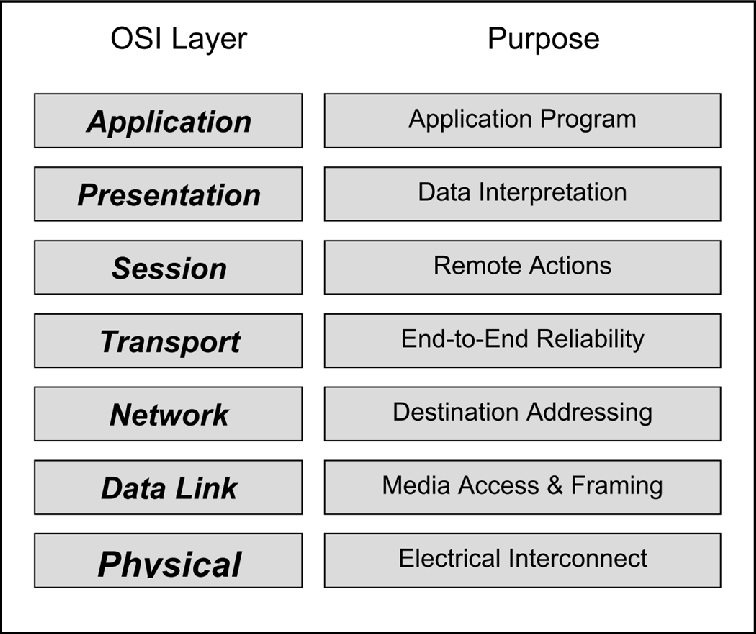
\includegraphics[scale=0.3]{The-layers-of-the-ISO-OSI-model-and-their-purposes-in-the-ISO-IEC-EN-14908-standard.png}
\subsection{Bandwidth}
The bandwidth also called (network bandwidth or data bandwidth) is measured as the amount of data that transferred from a one point to another within the same network over a fixed amount of time. Bandwidth is typically expressed as bitrate and calculated in bits per second (bps).\\
it's calculated by : $maximumdatarate\leq bandwith\log_{2} \frac{signal strength}{noise level} bits/sec$

The term bandwidth refers to the communication power of a link and is an important component in assessing the efficiency and speed of a network or internet service. 

There are a number of different ways to measure bandwidth. Some measurements are used to calculate the current data flow, while others measure the maximum data transfer rate over a given path.
bandwith used in many fields like signal processing, wireless communications and modem data transmission. \cite{7}

 \subsection{VPN}
 A virtual private network, or VPN, allows you to create  an encrypted connection over the Internet from a device to a network. The encrypted connection allows users to receive and send  data across any networks. It prevents unauthorizations people from eavesdropping on the traffic and allows the user to conduct work remotely with security, and management of the private network. VPN technology is used mainly in corporate environments. usually vpn connections are encrypted.
 \subsection{Network bridge}
 A network bridge is a computer network interface that generates a single network between various OSI Level 2 transmission networks, and it's a local area network ( LAN) data link layer. Routing permits several networks to communicate independently and yet remain separate, while bridge connects two separate networks to be a single network. Bridges will connect as LAN protocols, and bridged networks must transfer packets of higher-layer protocols that running on the network. Although any LAN interface can be bridged, the vast majority of LANs today are Ethernet switching LANs, and most of the bridges are Ethernet bridges.\cite{8}
 
\subsection{Repeater}
A repeater (also known as signal boosters and range extenders) is a network device used to recover or reproduce a signal. Repeaters are used in transmissions to regenerate analog or digital signals that are distorted by transmission loss and to re-transmit them to locations where Ethernet or Wi-Fi data transmissions can not be reached. Analog repeaters can also only amplify the signal and digital repeaters can transform the signal to close its original level. Repeaters aim to maintain the integrity of the signal and increase the distance over which the signals can pass. \cite{9}
\subsection{Router}

The router is a hardware networking device designed to sustain, analyze and move incoming packet from one network to another. Routers execute traffic control roles on the Internet. It can also be used to pass packets to another network gateway, remove them, move from one router to another router across the networks before it reaches its destination node.\cite{10}

\section{Network Design}
Computer networks have unique different designs, the two basic forms being client or server and peer-to - peer networks. Client or server networks have centralized storage servers that are accessed by client computers and devices.
There are several various types of network links that refer to how the network components are linked to each other. Topologies are used to link computers, with the most common form of collapsed ring owing to Ethernet connectivity for the internet, local area networks and wide area networks. 
Here are some of the topologies that are used to create a network:
\subsection{Star Topology}
The central node connects the cable to each computer on the network in the star topology .   Each computer in the network has an independent connection to the center of the network, and the rest of the network will not be affected by a single connection. One downside, however, is that several cables are needed to shape this kind of network.
\subsection{Bus Topology}


A single cable links the device to the bus topology network. The details for the last node on the network will pass through each attached computer. Less wiring is required, but if the cable breaks, it means that none of the computers can reach the network.
\subsection{Ring Topology}

Ring topology is nearly similar to the bus topology . It uses a single cable with nodes connected to each other so the signal can circulate through the network to find its recipient. Even when the network node is not operating properly, The signal will always attempt to reach its destination. The ring has a central node as a main node, a hub, a router/switch. The device has an ring topology and places for the cable to be plugged in. Every computer on the network has a private cable to connect to the device. so In any office, we get a hardware closet where all the machines are attached to the cabinet and the connection. \cite{6}

\section{Wired and Wireless Networks}

There are hunderds of protocols that can work with both wired/wireless networks.The Ethernet network uses either a twisted copper pair or a coaxial transmission system. The most widely used Ethernet cable is an unshielded twisted pair (UTP) cable—which is useful for companies that wants to connect various devices together, such as computers, scanners and printers, but it's less practical in home use because it's is bulky and costly . But A telephone line simply uses existing telephone wiring found in all homes and can provide fast  internet services such as ADSL. Eventually, Broadband networks can provide a broadband Internet service and use the same coaxial cable to provides us with cable television. However, The simplest, cheapest way to connect your home computers is to use a wireless network (WI-FI) that uses radio waves instead of cables. The lack of actual cables makes this network very flexible. The downside is that wireless connections are generally slower than Ethernet connections and they are less secure unless you take measures to protect your network. due to it's Easiness, wireless technologies have grown and become much more popular due to its flexibility .wireless technologies like Wi-Fi have become the a popular way to build networks. One reason for this is that wireless networks supports various types of wireless gadgets that have become popular over the years, such as smartphones, tablets and smart watches. Wireless networking is an important connection method , and it won't go anywhere any time soon. \cite{11}
\section{types of area network}
\subsection{LAN}
The LAN links network machines over relatively short distances. A networked office building, school, or home usually consists of a single LAN, although sometimes one building contains a few small LANs (maybe one per room) and occasionally a LAN encompasses a group of nearby buildings. For TCP / IP networking, LANs are mostly, but not necessarily, configured as a single IP subnet. 

In addition to operating in a limited area, LANs are also typically owned , controlled and managed by a single person or organization. These networks also tend to use certain connectivity technologies, in particular Ethernet and Token Ring.
\subsection{MAN}
 MAN or Metropolitan Area Network occupies a wider area than the LAN and a smaller area than the WAN. It links two or more computers that are independent but live in the same or different cities. This spans a wide metropolitan area and can act as an ISP ( Internet Service Provider). MAN is planned for consumers in need of high-speed networking. MAN speeds range at Mbps . It's hard to build and manage a network for the Metropolitan Region. 

The error acceptance of the MAN network is smaller and there is also more noise in the network and costly. The data transfer and the delay in the distribution of the MAN are low. Devices used to transmit data through a MAN network are: modem and wire / cable. Examples of a MAN are those parts of a telephone service network that can provide a high-speed DSL line to the consumer or cable TV network in a region.
\subsection{WAN}
WAN covers a great physical distance. The Internet is the largest WAN in the world. 

WAN is a dispersed groups of LANs. A network computer called a router links LANs to a WAN network. Through IP networking, the router holds LAN and a WAN address. 

WAN varies from LAN in a variety of essential respects. Most WANs (like the Internet) are not operated by a single entity. Instead, WANs live under mutual or delegated ownership and control. 

WANs prefer to use systems such as ATM, Frame Relay and X.25 for communication over longer distances.
\subsubsection{WLAN}
WLAN is a wireless computer network connecting two or more wireless networking devices to form a local area network ( LAN) within a small location, such as a residence, classroom, computer room, campus or office building. This allows people the freedom to travel about inside the field and remain connected to the network. The WLAN will also have a link to the broader Internet as a gateway. \cite{11}
\section{Routing}

Routing is a process that is performed by layer 3 network devices to deliver internet packet by choosing the best path from one network to another. 

There are three types of routing: 
\subsection{static routing}
Static Routing is a method by which we connect manually  routes to the routing list. 
Benefits – 
No overhead router for the CPU router, which means that a normal router can be used to route. 
Additional security because only the admin can allow routing to specific networks only. 
No use of bandwidth between routers. 
Disadvantage  
tough job for the admin to manually add every route to the network in the routing table for a large network. 
The admin is supposed to have strong understanding of the topology. When a new administrator arrives, he needs to manually connect each route


\subsection{Default Routing}

This is the mechanism by which the router is designed to deliver all packets to a single router .  No matter which network the packet belongs to, it is forwarded to a router that is configured for default routing. It's commonly used with stub routers. The Stub Router is a router that has only one path to access the other networks.
\subsection{Dynamic Routing}
Dynamic routing regularly updates the routes according to the current route state in the routing table. Dynamic routing uses protocols to identify network destinations and paths to access them. RIP and OSPF are the latest examples for dynamic routing protocols. Automatic modifications can be made to the path of the network if one route goes down.

The dynamic protocol has the following features: 

Routers would have the same dynamic protocol running to swap routes. 
When a router detects a difference in the topology, the router advertises it to all other routers.
Benefits – 

Easy to set up. 
More effective in selecting the best route to a remote network destination and also in discovering a remote network. 
Disadvantage of – 

Consumes more bandwidth to communicate with other neighbors. 
less protection than static routing.
\subsection{Routing Table}
The routing table is a series of rules, often presented in table format, used to decide where data packets moving over the Internet Protocol ( IP ) network should be led. Use routing tables for all IP-enabled devices, including routers and switches. See the routing table below:
\begin{table}[h]
\centering
\begin{tabular}{l l l}
\hline
\textbf{Destination} & \textbf{Subnet mask} & \textbf{Interface}\\
\hline
128.73.42.0   &   255.255.255.127   &    Eth0 \\
128.74.41.0   &   255.255.255.128  &    Eth1 \\
192.12.17.5   &   255.255.255.255   &   Eth3 \\
\hline
\end{tabular}
\caption{Table caption}
\end{table} \cite{3}

\section{Conclusion}
In conclusion, the networks span all facets of life: molecular, physical and social. They are indispensable to the functioning of the global economy. Globally, wireless connectivity is something that people should expect as technology progresses. Wireless communications have many advantages and can make the world more efficient. Computer communication in general will become a much more useful networking tool when a large number of people with similar interests have access to technology. Although it can accelerate the development of new interpersonal networks by overcoming the space and time barriers faced by traditional networking techniques,It also takes a lot of concerted energy and money to get people to use it. In the coming years, this issue will be gradually reduced as technical advances become more prevalent in society.


\begin{thebibliography}{10}
    \bibitem{1}
	Sutton, C., 2004. Internet Began 35 Years Ago At UCLA With First Message Ever Sent Between Two Computers Forum To Mark Anniversary Set For October 29. engineer.ucla. Available at: http://www.engineer.ucla.edu\\/stories/2004/Internet35.html .
	\bibitem{2}	
	Gillies, J., \& Cailliau, R. (2007). How the web was born. Oxford: Oxford University Press.
	\bibitem{3}
	Comer, D. E.,\& Droms, R. E. (2003). Computer networks and internets. Prentice-Hall, Inc..
	\bibitem{4}
	  Fisher,T. (2020) Understanding How a Switch Works in a Computer Network.b Retrieved 6 June 2020, from https://www.lifewire.com/definition-of-network-switch-817588
	  
	  \bibitem{5}
	  
	  What Is a Modem in Computer Networking?. (2020). Retrieved 6 June 2020, from https://www.lifewire.com/what-is-a-modem-817861
	
	\bibitem{6}
	Farrel, A. (2004). The Internet and its protocols. Amsterdam: Morgan Kaufmann Publishers.
	
\bibitem{7}
	Rouse, M. (2020). What is Bandwidth and How is it Measured?. Retrieved 6 June 2020, from https://searchnetworking.techtarget.com/definition/bandwidth
	
	\bibitem{8}
	Mitchell, B. (2020). What Is a Bridge in Computer Networking?. Retrieved 6 June 2020, from https://www.lifewire.com/how-network-bridges-work-816357
	
	\bibitem{9}
	What is a Network Repeater? (with pictures). (2020). Retrieved 6 June 2020, from https://www.wisegeek.com/what-is-a-network-repeater.htm
	
	
	\bibitem{10}
	All About Routers. (2020). Retrieved 4 June 2020, from http://www.practicallynetworked.com/networking/routers\_switches\_hubs.shtml




\bibitem{11}
	Hellberg, C., Greene, D., \& Boyes, T. (2007). Broadband network architectures. Upper Saddle River, NJ: Prentice Hall.
	
	
	
	
	
	
	\end{thebibliography}




%\bibliography{References}

\end{document}